\label{sec:cad}

\subsection{Scope of the Mechanical Design}
The mechanical side of the project is focused on the pistol grip, since that is where
all of the electronics for the Smart Trigger will live. Fitting everything inside a grip
gives us a very tight space to work with. The usable inner cavity of the grip measures
88.8\,mm from top to bottom, 21.9\,mm wide, and 45.0\,mm long. To put that in perspective,
the Raspberry Pi Pico W alone is 51\,mm long and 21\,mm wide, which leaves less than a
millimeter of room on either side of it in the width direction and means it can only
be oriented running from the top of the grip to the bottom. Every board, the motor,
the antenna, and the wiring between them all have to share this space.

With that in mind, the mechanical design is built around three main goals: size, secure
mounting, and usability. All of the electronics, including the
Pico W, the RDM6300 RFID reader, the SAA1042 motor driver, the micro stepper motor, and
the antenna, must fit within the 88.8\,mm $\times$ 21.9\,mm $\times$ 45.0\,mm inner
cavity of the grip. Fitting the boards inside the
grip is not enough on its own, as they also need to be held firmly in place so they are not
sliding around. A firearm sees a lot of shock and vibration from recoil and
normal handling, so the mounting has to hold up even after extensive use of the gun. A
loose board can break solder joints, pull wires, or shift the antenna away from where it
needs to be to read the tag. At the end of the day, the grip also
still has to be a usable and comfortable grip that mounts to a standard lower receiver
the same way a factory grip does.

\subsection{Custom Grip}
Instead of trying to fit our electronics into an off-the-shelf grip, we chose to design
and 3D print our own. Designing the grip ourselves gives us full control over the feel,
grip, and appearance of the final product. We can shape the inside around our boards
rather than shaping our boards around someone else's grip. We can also adjust the
outside profile so it stays comfortable in the hand even with a hollowed out core.
This also lets us place the RFID antenna exactly where we want it, close to where the
user's hand wraps around the grip so the ring tag stays within read range.

The other big benefit of a custom grip is how easy it is to iterate on. Because we are
printing the grips ourselves, a new version can go from a change in the model to a part
in our hands within the same hour. This means we can test fit, find a problem, fix it,
and print again without waiting on any outside vendor. For a project with as many
tight tolerances as this one, being able to prototype quickly is a huge advantage.

\subsection{Actuator Mount and Blocking Member}
As described in the Hardware Components and Integration section, our blocking method
works by locking the AR-15's native safety selector in place until an authorized user is
recognized. The stepper motor will be housed inside the grip and will rotate a shaft that
holds the safety selector in the safe position, then releases it once a valid tag is read.
Because the safety selector already sits right above the grip on the lower receiver, the
grip is a natural place to mount the motor close to it.

For now, the exact design of the actuator mount and blocking member is on hold until our
PCB arrives. Once we have the board in hand, we will connect everything together and
measure how the full assembly fits inside the grip. Those measurements will tell us how
much room is left for the motor and where it can be placed, so that the mount and blocker
can be designed around the real assembly instead of estimates.

\subsection{Materials and Print Parameters}
All of our grips are printed in PLA. PLA is cheap and easy to print, but it is still
resilient enough for the handling and fit testing we are doing at this stage of the
project. Since we expect to go through many versions of the grip before landing on a
final design, keeping the cost of each print low matters.

\subsection{Design Iteration}
Our grip design started from a standard AR-15 grip model, shown in
Fig.~\ref{fig:grip_original}. This model came in as a triangle mesh, which is good for
printing but difficult to edit. Making changes like hollowing out the inside or
reshaping a surface is tedious when the model is made up of thousands of small
triangles rather than clean faces.

\begin{figure} [h]
    \centering
    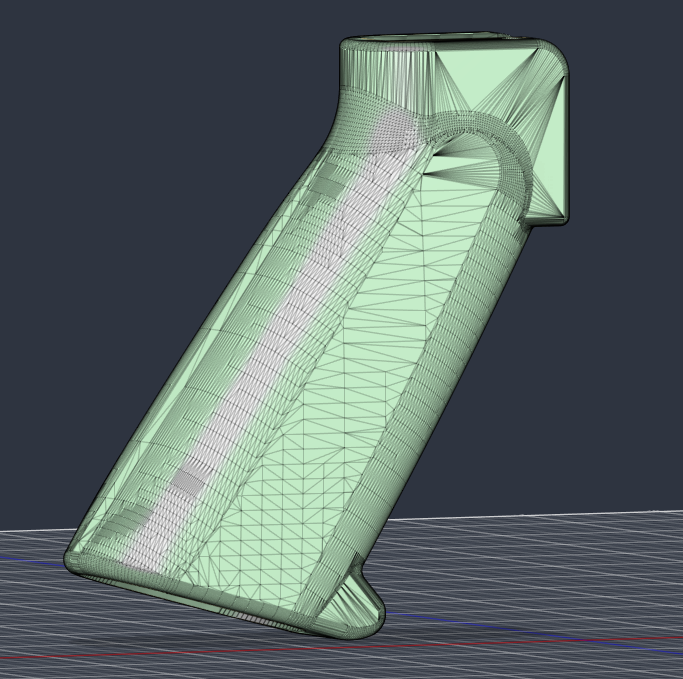
\includegraphics[width=0.35\textwidth]{Images/Grip_Iteration_Original.png}
    \caption{The original AR-15 grip model we started from. The model is a triangle mesh,
    which made it difficult to modify.}
    \label{fig:grip_original}
\end{figure}

For our newest iteration, shown in Fig.~\ref{fig:grip_current}, we first converted the
mesh into a solid body with clean, editable faces. With an editable model, we then
extruded the middle section of the grip outward. This gives us extended room inside the
grip to mount the board, and it also creates a flat surface on the exterior where the
RFID antenna is mounted. Putting the antenna on the outside of the grip keeps it as close
as possible to the user's hand and the ring tag, while keeping the inside free for the
electronics.

\begin{figure} [h]
    \centering
    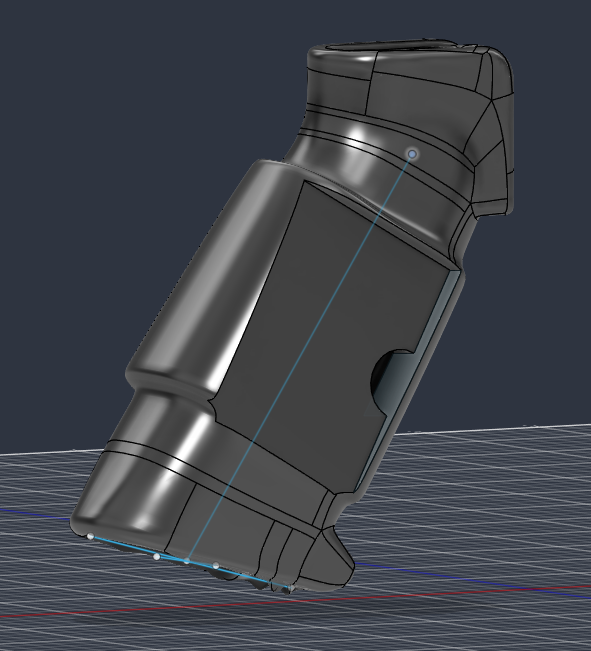
\includegraphics[width=0.35\textwidth]{Images/Grip_Iteration_Current.png}
    \caption{Our newest grip iteration. The model was converted to a solid body and the
    middle section was extruded outward to make room for the board inside and the RFID
    antenna on the exterior.}
    \label{fig:grip_current}
\end{figure}

The ideal final iteration will have housing for the boards and the motor built directly
into the inside of the grip. Rather than having the electronics sit loosely in a hollow
cavity, the inside of the grip will have slots and supports shaped to the board stack
and the motor so that each part is held in a fixed position. This will keep everything
secure through recoil and handling, keep the antenna in a consistent spot for reliable
tag reads, and make assembly simple, since each part will only fit one way. Getting to
that point depends on the measurements we will take once the PCB arrives, and with
prints only taking about an hour, we expect to work through several versions quickly
once we have them.